\subsection{Dokumenten-Management-Systeme}

Um ein Dokumenten-Management-System (\gls{DMS})  zu erläutern muss sich zuerst mit dem Begriff des \textbf{"`Dokuments"'} auseinander gesetzt werden.
In \cite{DMS08} S. 2 wird ein Dokument durch folgende Punkte definiert:

\begin{itemize}
\item Ein Dokument fasst inhaltlich zusammengehörende Informationen strukturiert zusammen, die nicht ohne erheblichen Bedeutungsverlust weiter unterteilt werden können. 
\item Die Gesamtheit der Information ist für einen gewissen Zeitraum zu erhalten.
\item Dokumente dienen oft dem Nachweis von Tatsachen.
\item Ein Dokument ist als Einheit ablegbar (speicherbar) und/oder versendbar und/oder wahrnehmbar (sehen, hören, fühlen).
\item Das Dokument ist eigentlich der Träger, der die Informationen speichert, egal ob das Dokument ein Stück Paper, eine Datei auf einem Rechner, ein Videoband oder eine Tontafel etc. ist. Dies bedeutet auch, dass es keine Bindung an Papier oder ein geschriebenes Wort gibt.
\end{itemize}

Desweiteren gibt es eine Differenzierung in zwei Definitionen:

\begin{quote}"`Als \textbf{Dokument im konventionellen Sinne} werden Dokumente bezeichnet, die als körperliches Dokumente (z. B. Papier) vorliegen, ursprünglich als körperliches Dokument vorlagen oder für die Publizierung auf einem körperlichen Medium vorgesehen sind.

Die Begrifflichkeit des \textbf{Dokuments im weiteren Sinne} erweitert den Begriff des Dokuments um semantisch zusammengehörende Informationsbestände, die für die Publikation in nicht-körperlichen Medien, z. B. Webseiten, Radio, Fernsehen o. ä. vorgesehen sind. Derartige Dokumente werden oft dynamisch gestaltet und zusammengestellt."' \begin{flushright}\cite{DMS08} S. 2\end{flushright}\end{quote}

Dabei müssen auch Daten und Dokumente voneinander abgegrenzt werden.
In \cite{DMS08} S. 33 werden Daten im Allgemeinen als eher stark strukturierte Informationen gesehen, wobei Dokumente zumeist aus unstrukturierte bis zu schwach strukturierte Informationen bestehen.
Eine eindeutige Klassifizierung eines vorhandenen Dokumentes lässt ist jedoch nicht immer möglich, da sich oft Mischungen beider Klassen finden (lassen).
Ohne die dazugehörigen Metadaten besteht ein (graphisches) Bild aus unstrukturierten Informationen, daher auch \gls{NCI}-Dokument für None-Coded Information genannt.
Der Anteil von strukturierten Informationen in einem Dokument nimmt von Bildern über Text zu Tabellen zu, da hier die Dokumente vollautomatisch auswertbar sind, siehe hierzu Abbildung ???.

\begin{center}
Bild \cite{DMS08} S. 33
\end{center}

Die Einordnung, wann ein Dokument strukturierte oder unstrukturierte Informationen enthält, lässt an folgenden Beispielen verdeutlichen.
Bei einem Bild oder Foto lassen sich die enthaltenen Informationen nicht durch Computer bestimmen.
Beispielsweise, ob sich eine Person auf dem Bild befindet oder wann und wo das Foto erstellt wurde.
Daher ist ein Bild, solange keine Metadaten darüber bekannt sind, ein eindeutiges Beispiel für \gls{NCI}-Dokumente mit unstrukturierten Informationen.
Im Gegensatz dazu lassen sich die Werte einer Tabelle oder eines Datensatzes durch die Spaltennamen eindeutig bestimmen und durch den Computer auslesen.
Solche Daten mit strukturierten Informationen werden daher auch als Dokumententyp mit Coded Information (\gls{CI}) bezeichnet.

Unter \textbf{Dokumenten-Management} werden primär die Verwaltungsfunktionen Erfassung, Bearbeitung, Verwaltung und Speicherung von Dokumenten verstanden. \cite{DMS08} S. 344.

Darunter fallen laut \cite{DMS08} S. 3 folgende Punkte:

\begin{itemize}
\item Kennzeichnung und Beschreibung von Dokumenten (auch Metadaten des Dokuments genannt) 
\item Fortschreibung, Versionierung und Historienverwaltung von Dokumenten
\item Ablage und Archivierung von Dokumenten
\item Verteilung und Umlauf von Dokumenten
\item Suche nach Dokumenten bzw. Dokumenteninhalten
\item Schutz der Dokumente vor Verfälschung, Missbrauch und Vernichtung
\item Langfristiger Zugriff auf die Dokumente und Lesbarkeit der Dokumente
\item Lebenslauf und Vernichtung von Dokumenten
\item Regelung von Verantwortlichkeiten für Inhalt und Verwaltung von Dokumenten
\end{itemize}

Der Begriff \textbf{"`Dokumenten-Management-System"'} muss auch in zwei verschiedene Sichtweisen differenziert werden:
\begin{quote}"`Bei \textbf{Dokumenten-Management-Systemen im engeren Sinne} geht es um die Logik der Verwaltung von Dokumenten, deren Status, Struktur, Lebenzyklus und Inhalt. Dokumente werden beschrieben, klassifiziert und in einer bestimmten logischen Struktur eingeordnet, damit sie einfach wieder gefunden werden können. Dokumente entstehen, werden verändert und (irgendwann) vernichtet.

Den \textbf{Dokumenten-Management-Systemen im weiteren Sinne} ordnet man auch noch weitere Funktionalitäten zu, wie z. B. Schrifterkennung, automatische Indizierung, [...], Publizierung. Hier lassen sich die Grenzen nicht mehr genau bestimmten!"' \begin{flushright}\cite{DMS08} S. 5\end{flushright}\end{quote}

Die Grundstruktur eines Dokumenten-Management-Systemes kann man dadurch grob in folgender Abbildung zusammenfassen:

\begin{center}
Bild \cite{DMS08} S. 38
\end{center}

Dabei wird ein DMS-System in drei verschiedene Teilbereiche aufgegliedert:

\subsubsection{Eingabe}
Unabhängig des Ursprungs oder der Art des Dokumentes besitzt der Funktionsbereich Eingabe die Aufgabe diese Dokumente dem Dokumenten-Management-System zuzuführen.
(Darunter fallen auch Post, Email, Andere anwendungen, fax usw. - Hier Hinweis auf WSDL)

Laut \cite{DMS08} S. 40fff fallen in diesen Bereich zwei Funktionen:

\paragraph{Dokumenteneingang}
Hier wird die Zuspielung der Dokumente in das DMS-System durch verschiedene Methoden behandelt / realisiert.
Als mögliche Eingabe von Dokumenten kann sowohl das Einscannen von Textdokumente oder Bilder als auch der elektronische Eingang von Dokumenten durch E-Mail oder externen Anwendungen fungieren.

Auch hier gilt zu unterscheiden, dass durch den Einscannvorgang erstellte Dokumente als \gls{NCI}-Dokument abgelegt werden und bereits digitalisierte Dokumente sich zur Umwandlung zu \gls{CI}-Dokumenten anbieten.
Sobald der Inhalt von eingescannten Dokumenten zur weiteren Verarbeitung ausgelesen bzw. ausgewertet werden soll, müssen die Dokumente in ein \gls{CI}-Format transformatiert werden.
Dies wird häufig durch eine \gls{OCR}-Software realisiert, die beispielsweise das Bild eines eingescannten Briefes in (bearbeitbaren) Text umwandelt.

Bereits im \gls{CI}-Format vorliegende Dokumente müssen nicht transformiert werden, jedoch werden die Dokumente oft in anderen Formaten zusätzlich abgespeichert.
Ein Beispiel ist die Umwandlung eines Microsoft Word-Dokumentes in ein \gls{PDF}-Dokument oder von unterschiedlichen Bildformaten in ein einheitliches Format.

\paragraph{Indizierung}
Bei der Indizierung werden Dokumente zur eindeutigen Identifikation mit Attributen versehen.
Diese Attribute werden teilweise autonomisch durch das DMS-System anhand einer hochzählenden Identifikationsnummer oder manuell durch den Benutzer beim Einstellen des Dokumentes hinzugefügt.
Solche Attribute werden auch als Metadaten des Dokumentes bezeichnet und meist als zusätzliche Suchkriterien angeboten.

Dabei werden in \cite{DMS08} S. 44 zwei verschiedene Methoden zur automatischen Klassifizierung genannt.
Beim wissenbasiertem Ansatz wird mittels umfangreichem Wissen über das Umfeld der Dokumente und dadurch abgeleitete Regeln dem System ermöglicht diese Dokumente automatisch einzuordnen und zu indizieren.
Eine weitere Möglichkeit eröffnet sich durch das Verwenden von neuronalen Netzen.
Hierbei wird durch die Vorarbeit eines Menschen Beispiele geschaffen anhand welcher sich das System selbstständig (Auswahl)Kriterien erzeugt.
Je mehr korrekte Beispiele vorgegeben werden, desto besser und zuverlässiger arbeitet die automatische Klassifizierung.

\subsubsection{Verwaltung und Archivierung}
Bei der \textbf{Verwaltung} werden die Probleme beim \textit{Check-in} (Einspielen des Dokumentes), Bearbeitung und \textit{Check-out} (Signalisierung der Weiterbearbeitung) behandelt, siehe auch Abbildung \cite{DMS08} S. 38 ???.
Wie auch bei einer Datenbank müssen Dokumente, die gerade bearbeitet werden, für andere Benutzer für Änderungen gesperrt werden, damit keine Inkonsistenzen auftretten können.
Nach einer Bearbeitung und dem Check-in des abgeänderten Dokumentes muss die Versionsverwaltung des DMS-Systems beide Versionen beibehalten und (dabei) die ursprüngliche Version als veraltet und die neue Version als solche kennzeichnen.
Zusätzlich muss die Wiederherstellung einer älteren Revision als aktuelles Dokument unterstütz werden.


Die \textbf{Archivierung} befasst sich mit der Sicherung und Wiederherstellung von Dokumenten und deren Metadaten.
Im Zusammenhang mit DMS-Systemen springt man auch von einer revisionssicheren Archivierung.
Dabei müssen laut \cite{DMS08} S. 288 unter anderem bestimmte Punkte beachtet / eingehalten werden:

\begin{itemize}
\item Jedes Dokument muss unveränderbar archiviert werden.
\item Es darf kein Dokument auf dem Weg ins Archiv oder im Archiv selbst verloren gehen.
\item Kein Dokument darf während seiner vorgesehenen Lebenszeit zerstört werden können.
\item Jedes Dokument muss in genau der gleichen Form, wie es erfasst wurde, wieder angezeigt und gedruckt werden können.
\end{itemize}

\subsubsection{Ausgabe}
Wie die Eingabe besteht die Ausgabe aus zwei Funktionen:

\paragraph{Recherche}
Die Recherche ist die Suche nach einem Dokument entweder durch eine strukturierte Suche anhand von zuvor eingetragenen Attributen (Author, Erstellungsdatum, Speichergröße usw.) oder durch eine Volltextsuche.

Die \textbf{strukturierte Suche} ist nur bei einer qualitativ hochwertigen Indizierung effizient, bietet dafür auch mit guter zeitlichen Performanz die besten / genauersten Ergebnisse, sofern die Indizierung entsprechend aufgebaut / eingehalten wurde.

Die \textbf{Volltextsuche} durchsucht "`stupide"' den Inhalt der Dokumente nach den eingegebenen Suchbegriffen.
Daher ist die Qualität der Suchergebnisse unabhängig von der Qualität der Indizierung.
Jedoch können nur \gls{CI}-Dokumente, deren Informationen auch durch den Computer auslesbar und interpretierbar sind, durchsucht werden.
\gls{NCI}-Dokumente wie Bilder oder Videos können durch die Volltextsuche nicht gefunden werden.

\paragraph{Reproduktion}
In diesem wichtigem Teilbereich können die gespeicherten Dokumente wieder vom Benutzer abgerufen werden.
Dies ist durch eine einfach Anzeige im Webbrowser, eine Weiterleitung per E-Mail oder eine Sendung als Druckauftrag möglich.



\subsection{Content-Management-Systeme}
Bei einem Content-Management-System (\gls{CMS})  steht nicht mehr das eigentliche Dokument im Vordergrund, sondern vielmehr der enthaltene Informationsgehalt des Dokuments.
Der Unterschied zwischen einem \gls{DMS} und einem \gls{CMS} besteht laut \cite{DMS08} S. 114 im/in Folgenden/m:

\begin{quote}"`Abgrenzend zum Dokumenten-Management handelt es sich beim Content-Management nicht vordergründig um die Verwaltung von Dokumenten, sondern um die Verwaltung von Informationseinheiten, die miteinander verknüpft sein können. [...] Je nach Ausprägung kann nun ein konkretes System als Dokumenten-Management-System mit Content-Management-Funktionen definiert werden und umgekehrt. [...]
Der Ansatz des Content-Management unterscheidet sich vom "`klassischen"' Dokumenten-Mangement vor allem in Bezug auf die betrachteten Objekte: Ein DMS hat als kleinestes Objekt der Betrachtung eines einzelnen Dokument. [...] Content-Management ist auf logische Informationseinheiten ausgerichtet. Es ist z.B. das Ziel des Content-Managements, Inhalte, die auf mehrere Quellen verteilt sind, neue zusammenzustellen und daraus z.B. ein neues Dokument zu generieren."'
\begin{flushright}\cite{DMS08} S. 114f\end{flushright}\end{quote}

Die folgende Abbildung soll den (charakteristischen) Unterschied zwischen CMS-Systemen und DMS-Systemen verdeutlichen.

\begin{center}
Bild \cite{DMS08} S. 115
\end{center}

Wie zuvor beschrieben ist die Sichtweise eines DMS nur auf die einzelnen Dokumente beschränkt, während ein CMS einzelne Elemente / Informationen aus den Dokumenten extrahieren und ggf. zu einem neuen Dokument verschmelzen kann. Die Sichtweise des CMS wird durch das gestrichelte Polygon dargestellt, welches hier dokumentenübergreifend abgebildet ist.

Der (theoretische/beabsichtigte) Zweck, weshalb ein CMS-System eingesetzt wird, ist laut Oracle folgendermaßen definiert:

\begin{quote}"`The key to a successful content management implementation is unlocking the value of content by making it as easy as possible for it to be consumed. This means that any piece of content must be available to any consumer, no matter what their method of access."'
\begin{flushright}\cite{UCM07} S. 12\end{flushright}\end{quote}

Ein CMS soll die Informationen jedes/jedwedem (Inhalts) extrahieren/aufnehmen und jedes Einzelteil / Element dieser Information den Benutzern zugänglich machen, unabhängig von der Art des Zugriffs.
Dieses Konzept soll in Abbildung \ref{ucm-a2a} verdeutlicht werden.

\begin{figure}[ht]
	\centering
	   \fbox{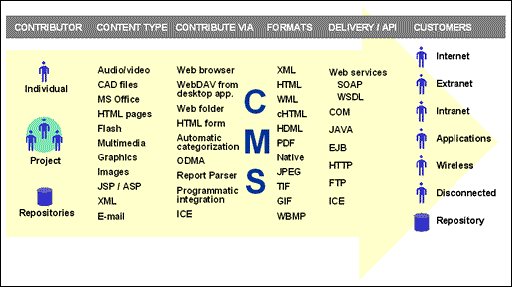
\includegraphics[width=0.95\textwidth]{bilder/ucm.png}}
		\caption["`any-to-any"' Content-Management Konzept]{"`any-to-any"' Content-Management Konzept\protect\footnote}
		\label{ucm-a2a}
\end{figure}
\footnotetext{Quelle: \cite{UCM07} S. 12}

Das CMS steht hier in der Mitte der Abbildung als Medium zwischen den verschiedenen Inhalten, eingestellt von den \textit{Contributors} (links), und den Anwendern, die auf transformierte Versionen der Inhalte durch unterschiedliche Arten zugreifen (rechts).


\subsection{[Enterprise-Content-Management-Systeme]}
In diesem Zusammenhang / Kontext sei auch der Begriff Enterprise-Content-Management (\gls{ECM}) genannt.
Laut der "`Association for Information and Image Management"' (\gls{AIIM}\footnote{Die AIIM ist eine Gesellschaft von internationalen Herstellern und Anwendern von Informations- und Dokumenten-Mangement-Systemen}), welche sich mit umfasst dieser Begriff die Verwaltungfunktionen von Unternehmensinformationen in unterschiedlichen Dokumentformaten.\footnote{Quelle: \url{http://www.aiim.org/What-is-ECM-Enterprise-Content-Management.aspx}}
Diese Funktionen werden laut \cite{DMS08} S. 116 durch verschiedene "`Systeme wie Dokumenten-Management, Groupware, Workflow, Input- und Output-Management, (Web-)Content-management, Archivierung, Records-Management und andere"' bereitsgestellt.


\subsection{Universal-Content-Management-Systeme}
Im Gegensatz zu anderen CMS-Systemen, wie Typo3 oder Joomla, bezeichnet Oracle seine Softwarelösung in diesem Bereich als Universal-Content-Management (\gls{UCM}).
Jedoch unterscheidet es sich in der technisches Umsetzung nicht von anderen CMS-Systemen.
Es wir vermutet, dass sich Oracle durch diese Bezeichnung von den anderen CMS-Systemem abheben / absetzten wollte, also nur aufgrund von Marketing-Vorteilen ihr Produkt so nannte.




















